\documentclass[11pt]{scrartcl}
\usepackage[sexy]{evan}
\usepackage{color}
\usepackage{fancyhdr}
\usepackage{float}
\usepackage{longtable}
\usepackage[normalem]{ulem}
\useunder{\uline}{\ul}{}
\usepackage{longtable}
\usepackage{hyperref}

%\Newassociation{sketch}{hintitem}{hints}
%\renewcommand{\solutionextension}{out}
\usepackage[none]{hyphenat}
%\usepackage[margin=1in]{geometry}
\newcommand\EE{\mathbb E}
\newcommand\PP{\mathbb P}
%\setlength{\parindent}{0em}
%\setlength{\parskip}{2.5em}

\definecolor{dkgreen}{rgb}{0,0.6,0}
\definecolor{gray}{rgb}{0.5,0.5,0.5}
\definecolor{mauve}{rgb}{0.58,0,0.82}
\definecolor{ChadDarkBlue}{rgb}{.1,0,.2}  
\definecolor{ChadBlue}{rgb}{.1,.1,.5}  
\definecolor{ChadRoyal}{rgb}{.2,.2,.8}  
%\definecolor{ChadGreen}{rgb}{0,.35,.1}
%\definecolor{ChadGreen}{rgb}{0,.5,.25}  % Too bright
%\definecolor{ChadGreen}{rgb}{0,.4,.2}    % Still too bright
\definecolor{ChadGreen}{rgb}{0.5, 0, 0.2}    % Dark Green
%\definecolor{ChadRed}{rgb}{.8,.1,.2}    % Too bright
\definecolor{ChadRed}{rgb}{.5,0,.5}  % purple

\usepackage{authblk}
\author[1]{Ritika Bhakat}
\author[2]{Kusumita Pradhan}
\author[3]{Asmita Debbarma}
\author[4]{Pratyusha Roy}
%\author[2]{Corresponding Author\thanks{email@2nduniversity.com}}
\affil[1,2,3,4]{Indian Institute of Science Education and Research Kolkata}
{
	\makeatletter
	\renewcommand\AB@affilsepx{: \protect\Affilfont}
	\makeatother
	
	\affil[ ]{Email ids}
	
	\makeatletter
	\renewcommand\AB@affilsepx{, \protect\Affilfont}
	\makeatother
	
	\affil[1]{\mailto{rb21ms095@iiserkol.ac.in}}
	\affil[2]{\mailto{kp21ms101@iiserkol.ac.in}}
	\affil[3]{\mailto{ad21ms130@iiserkol.ac.in}}
	\affil[4]{\mailto{pr21ms007@iiserkol.ac.in}}
}

\title{\color{ChadBlue}Impact of COVID - 19 on Education: \texttt{A case study on $1^{st}$ year students of IISER Kolkata}}
\date{\today}

\pagestyle{fancy}
\fancyhead{}
\fancyfoot{}
\fancyhead[C]{\MakeUppercase{HU1203: Sociology Project}}
\fancyfoot[C]{\thepage}

\begin{document}
	\maketitle
	
	\begin{abstract}
		\sffamily\small
		
	\end{abstract}
	\vfill
	\begin{figure}[H]
		\centering
		
\includegraphics[scale=0.2]{logo}
	\end{figure}
	
	\pagebreak
	
	\thispagestyle{empty}
	\tableofcontents
	\thispagestyle{empty}
	\clearpage
	
	\setcounter{page}{1}
	
	\section{Acknowledgements}
	
	We would like to sincerely thank the following people who made valuable contributions to the development of this case study:
	\begin{enumerate}
		\item Our batchmates who participated in this survey and shared their experiences during the pandemic and shared their unique experiences of learning continuity during this pandemic.
		
		\item Our professor Sujata Sen for providing us with such interesting and influential topic to work with. We got to work on field and in-depth about the problems that students went through during the pandemic.
		
		\item Finally, we would again wish to express special appreciation to professor Sujata Sen for providing us the time and making us indulge in the production of this report. 
	\end{enumerate}
	
	\pagebreak
	
	\section{Introduction}
	
	Coronaviruses are a  group of enveloped viruses with non-segmented,  single-stranded,  and positive-sense RNA 
	genomes. Apart from infecting a variety of economically important vertebrates (such as pigs and chickens), six 
	coronaviruses have been known to infect human hosts and cause respiratory diseases. Among them, severe acute 
	respiratory syndrome coronavirus (SARS-CoV) and Middle East respiratory syndrome coronavirus (MERS-CoV) 
	are zoonotic and  highly  pathogenic  coronaviruses  that  have  resulted  in  regional  and  global  outbreaks 
	Coronaviruses possess a distinctive morphology, the name being derived from the outer fringe,  or “corona” of the embedded envelope protein. Members of the family Coronaviridae cause a broad spectrum of animal and human diseases. Human coronavirus (HCoV) infection causes respiratory diseases with mild to severe outcomes.
	
	The COVID-19 pandemic has not stopped at national borders. It has affected people regardless of nationality, level of education, income or gender.
	The COVID-19 pandemic has also had a severe impact on higher education as universities closed their premises and countries shut their borders in response to lockdown measures. Although higher education institutions were quick to replace face-to-face lectures with online learning, these closures affected learning and examinations as well as the safety and legal status of international students in their host country. Perhaps most importantly, the crisis raises questions about the value offered by a university education which includes networking and social opportunities as well as educational content. To remain relevant, universities will need to reinvent their learning environments so that digitalisation expands and complements student-teacher and other relationships.
	
	Reopening schools and universities would bring unquestionable benefits to students and the wider economy. In addition, reopening schools would bring economic benefits to families by enabling some parents to return to work. Those benefits, however, must be carefully weighed against the health risks and the requirement to mitigate the toll of the pandemic.
	
	The reason behind choosing this topic as our dissertation project is that we have experienced the whole covid pandemic, The shutdown of school, lockdown, initiation of online classes, the drawbacks and the benefits of online learning, and the problems one can face while studying without proper interaction with teachers and peers. It is definite that everyone who experienced this pandemic will have a different view for the online mode of learning, this project is the best way to collect everyone’s experience and bring it in front of us.
	
	\pagebreak
	
	\section{Literature Review}
	
	This section proceeds along keeping the objective of the study in view. On 31 December 2019, WHO was informed of cases of pneumonia of unknown cause in Wuhan City, China. A novel coronavirus was identified as the cause by Chinese authorities on 7 January 2020 and was temporarily named “2019-nCoV”.
	
	Coronaviruses (CoV) are a large family of viruses that cause illness ranging from the common cold to more severe diseases. A novel coronavirus (nCoV) is a new strain that has not been previously identified in humans. The new virus was subsequently named the “COVID-19 virus”.
	
	The coronavirus disease (COVID-19) pandemic has caused an unprecedented crisis in all areas. In the field of education, this emergency has led to the massive closure of face-to-face activities of educational institutions in more than 190 countries in order to prevent the spread of the virus and mitigate its impact.
	The Economic Commission for Latin America and the Caribbean (ECLAC) has argued that even before the pandemic hit, the social situation in the region was deteriorating, owing to rising rates of poverty and extreme poverty, the persistence of inequalities and growing social discontent. In this context, the crisis will have a profoundly negative impact on the various social sectors, particularly health and education, as well as on employment and poverty. Meanwhile, UNESCO has identified major gaps in educational outcomes, which are related to the unequal distribution of teachers in general, and of the best qualified teachers in particular, to the detriment of lower-income countries and regions and of rural areas, where indigenous and migrant populations tend to be concentrated.
	
	In the sphere of education, many of the measures that the region’s countries have adopted in response to the crisis are related to the suspension of face-to-face classes at all levels, which has given rise to three main areas of action: the deployment of distance learning modalities through a variety of formats and platforms (with or without the use of technology); the support and mobilization of education personnel and communities; and concern for the health and overall well-being of students.
	
	\begin{figure}[H]
		\centering
		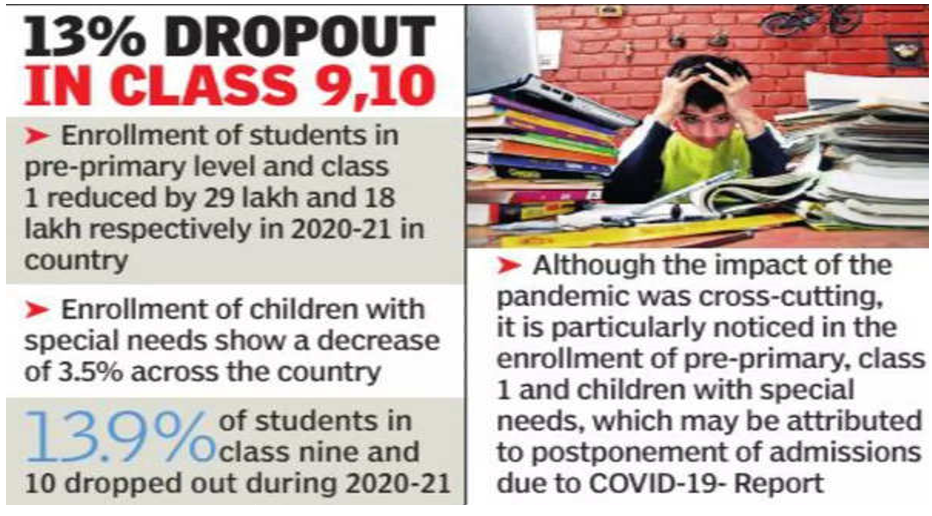
\includegraphics[scale=0.6]{pic1}
	\end{figure}

	\begin{enumerate}[$\bullet$]
		\item The COVID-19 has resulted in schools shut all across the world. Globally, over 1.2 billion children are out of the classroom.
		
		\item As a result, education has changed dramatically, with the distinctive rise of e-learning, whereby teaching is undertaken remotely and on digital platforms.
		
		\item Research suggests that online learning has been shown to increase retention of information, and take less time, meaning the changes coronavirus have caused might be here to stay.
	\end{enumerate}
	
	\begin{figure}[H]
		\centering
		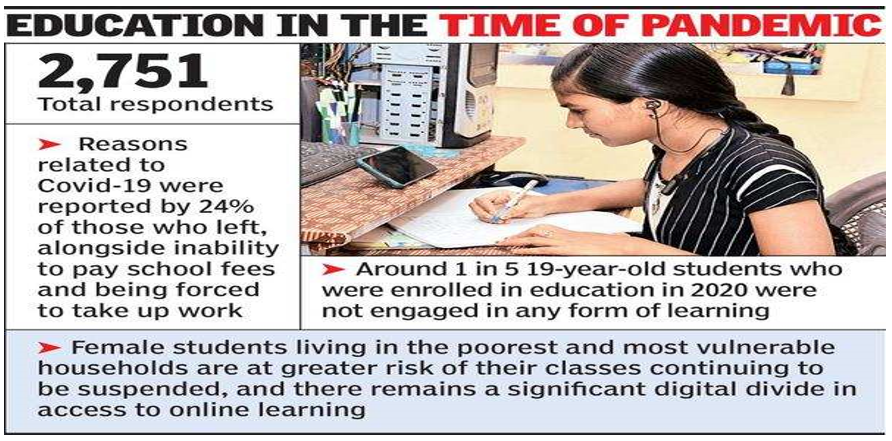
\includegraphics[scale=0.6]{pic2}
	\end{figure}
		
	The aim of this document is to shed light on various consequences that these measures will have on educational communities in the short and medium term, and to offer key recommendations on how to manage those consequences in the best possible manner, drawing attention to opportunities for learning and innovation in the post-pandemic education system.
	
	\pagebreak
	
	\section{Methodology}
	
	This section is devoted to the discussion of the methods that are put into use for the present study. Method provides the direction of the study. It sets the ‘why’ and ‘how’ of the research problem. In other words, this section highlights why this topic is selected and how the study is carried over. 
	
	We all know the sudden outbreak of a deadly COVID – 19 caused by a corona Virus (SARS-CoV-2) shook the entire world. It has affected people regardless of nationality, level of education, income or gender. But the same has not been true for its consequences, which have hit the most vulnerable hardest. Education is no exception. This crisis has exposed the many inadequacies and inequities in our education systems – from access to the broadband and computers needed for online education, and the supportive environments needed to focus on learning, up to the misalignment between resources and needs. 
	
	India is the second most impacted country in the world after the United States but with far fewer recorded deaths. Around 32 crore learners stopped to move schools/colleges and all educational activities halted in India. We felt curious to know the impact of the pandemic on higher education in India. Hence, we opted for this topic as the area of the present study. With this aim in view, we started collecting data. In addition to a literature review, we also involved case study. For this case study, we framed some relevant questions that we wish to ask our informants and interviews were held in June 2022 and reflect the experience of students up to this date. 
	
	The conversations provided opportunities to discuss the lessons learned and what remains to be done. We also relied on secondary data in order to obtain information related to the proposed study as it was not be possible for us to collect primary data on the area within such a short time period. It is relevant to point out that secondary data are such statistical information which have already been collected by someone for his own purpose and now are available for use by others for their purposes. ``Numerical data which are not gathered directly from the field of enquiry, but are merely compiled by other sources, are referred to as secondary data" (Das, NG: 2006). The chief sources of such data can be official publications of State or Central governments, international publications, journal papers and magazines, etc. 
	
	For the present work, we collected data from the articles published by UNICEF, WHO and various other publication sites. All these data have been collected by them with the help of statistical tools and quantitative methods. We, in order to observe the impact of COVID - 19, selected few relevant data from these sources that would serve our purpose. We accessed data, keeping the issue of their availability in mind. In some cases, however, in order to get a more thorough insight of the situation qualitative techniques like focus group discussion or case studies have been undertaken. After going through the data that we collected and secondary data, the next task was to analyse these relevant details . In conclusion, we attempted to provide a summary of our observations and some recommendations and suggestions in view of the pandemic. 
	
	The main objectives of our study are: 
	
	\begin{enumerate}
		\item To assess the rise and origin of deadly coronavirus.
		
		\item To which extent the deadly virus laid down cascading effect on education in India.
		
		\item To portray as to what extent the virus has affected the students.
		
		\item To recommend some measures.
	\end{enumerate}

	\pagebreak

	\section{Data Analysis}
	
	\begin{longtable}[c]{|l|l|l|l|l|}
		\hline
		Sl. No. &
		Name &
		\begin{tabular}[c]{@{}l@{}}How did the \\ pandemic \\ affect your \\ education?\end{tabular} &
		\begin{tabular}[c]{@{}l@{}}How did you\\  cope up \\ with the\\  stress due\\  to \\ online\\  learning ?\end{tabular} &
		\begin{tabular}[c]{@{}l@{}}What is your \\ opinion \\ about online \\ and offline \\ classes?\end{tabular} \\ \hline
		\endfirsthead
		%
		\endhead
		%
		1 &
		Aman Aryatosh &
		\begin{tabular}[c]{@{}l@{}}It affected\\  a lot.\end{tabular} &
		\begin{tabular}[c]{@{}l@{}}For coping \\ up with the \\ stress due \\ to online \\ learning \\ one needs \\ to study \\ which I \\ didn’t do \\ apparently.\end{tabular} &
		\begin{tabular}[c]{@{}l@{}}Offline classes \\ are way more \\ better than\\  online classes \\ according to \\ my opinion.\end{tabular} \\ \hline
		2 &
		Shreya Mukherjee &
		\begin{tabular}[c]{@{}l@{}}It had a negative\\  effect on\\ my education. \\ Stuck within \\ the walls of \\ our homes, \\ unable to go \\ to schools, \\ coaching etc. \\ social \\ interaction \\ with peers and \\ teachers became \\ negligible.\end{tabular} &
		\begin{tabular}[c]{@{}l@{}}I would \\ sit and \\ talk to \\ my \\ family \\ and I \\ love cooking \\ so I \\ would make \\ different\\ \\ dishes \\ for my \\ family and \\ occasionally \\ meditate \\ because \\ meditation\\  always \\ helps.\end{tabular} &
		\begin{tabular}[c]{@{}l@{}}Online classes \\ have become \\ a need in \\ today's time \\ but no \\ matter what \\ it could \\ never be \\ as good as \\ offline classroom \\ education. \\ The healthy \\ student-student and \\ student-teacher \\ interaction is \\ an absolute \\ necessity.\end{tabular} \\ \hline
		3 &
		Anusha Bannerjee &
		\begin{tabular}[c]{@{}l@{}}Surprisingly, the \\ pandemic \\ had a positive \\ effect on my \\ education \\ because I got a \\ lot more \\ time to study. \\ I \\ was able to \\ plan my day \\ efficiently and \\ study for \\ long periods \\ of time \\ without getting \\ physically \\ exhausted.\end{tabular} &
		\begin{tabular}[c]{@{}l@{}}Overall, online\\  learning \\ didn’t stress \\ me out. I \\ made time \\ to read books, \\ write, draw, \\ sing and\\  listen \\ to music.\end{tabular} &
		\begin{tabular}[c]{@{}l@{}}Offline classes \\ are much \\ better than \\ online classes \\ for obvious \\ reasons, like \\ meeting people, \\ improving \\ concentration \\ towards \\ studies, \\ and having \\ no negative\\  effect on the \\ health of \\ our eyes.\end{tabular} \\ \hline
		4 &
		Niveditha E. &
		\begin{tabular}[c]{@{}l@{}}The education \\ system \\ changed to \\ online, badly \\ affected health \\ due to \\ long screentime, \\ Missed \\ learning process, \\ book \\ reference \\ and group \\ discussions.\end{tabular} &
		\begin{tabular}[c]{@{}l@{}}Did my\\  favourite \\ hobbies \\ like dancing \\ and singing.\end{tabular} &
		\begin{tabular}[c]{@{}l@{}}Offline classes \\ are the \\ best \\ option\\  for education\\  as it \\ allows us\\  to interact \\ with \\ our friends \\ and take \\ studies \\ more enjoying.\end{tabular} \\ \hline
		5 &
		Sriparna Barman &
		\begin{tabular}[c]{@{}l@{}}For the pandemic,\\  I had to \\ face online \\ classes for \\ the  \\ first time \\ which became \\ very hectic \\ for me. \\ Attending\\  online \\ classes made \\ me mentally \\ tired affectedected \\ my \\ education.\end{tabular} &
		\begin{tabular}[c]{@{}l@{}}After classes \\ I used to \\ spend \\ my time in \\ the garden \\ listening \\ to soulful \\ music.\\  I used to \\ follow my\\  passion \\ which \\ kept me \\ better when \\ the day \\ was hectic.\end{tabular} &
		\begin{tabular}[c]{@{}l@{}}Online classes \\ save enough \\ time for \\ the students. \\ But we \\ can't explore \\ the lab and\\  do \\ experiments \\ through this,\\  also \\ it effects \\ our eyes. \\ In offline \\ education , \\ we can \\ clear our \\ doubts easily \\ without any \\ network issues.\end{tabular} \\ \hline
		6 &
		Deepshikha Singh &
		\begin{tabular}[c]{@{}l@{}}An adverse \\ affect on \\ me \\ was like\\  headache \\ eye pain \\ and also \\ due to online \\ classes I \\ don't \\ concentrate \\ that much \\ in the class \\ that \\ usually happens \\ in offline \\ classes. But \\ there was a \\ good \\ thing as well\\  I my technical \\ skills got better,\\  also I got \\ introduced \\ with many \\ new areas \\ I learnt many \\ new things.\end{tabular} &
		\begin{tabular}[c]{@{}l@{}}To cope up \\ with my\\  stress \\ I always \\ spend time \\ with \\ my parents \\ and family \\ members. \\ They always \\ gives me \\ the advice \\ to be \\ calm, I \\ played \\ games I \\ learnt \\ many new \\ things like i \\ learnt sketching, \\ crafting \\ and such \\ things.\end{tabular} &
		\begin{tabular}[c]{@{}l@{}}In online \\ classes we\\  interact \\ with teachers \\ friends we \\ develop \\ our concepts\\  more \\ \\ effectively \\ but at the\\  same \\ time we \\ get less time \\ to do \\ other things \\ in which \\ we are \\ interested. On \\ the other \\ hand \\ during online \\ classes, \\ we are \\ not that \\ much active \\ but we \\ usually \\ have much\\  more \\ time that \\ we can utilise \\ for self \\ improvement.\end{tabular} \\ \hline
		7 &
		Tanvi Shirude &
		\begin{tabular}[c]{@{}l@{}}The main \\ thing that \\ got affected \\ for me \\ was verbal \\ communication \\ and discussions \\ with professors \\ and batchmates. \\ Also mental \\ stress got \\ affected \\ to a certain\\  extent.\end{tabular} &
		\begin{tabular}[c]{@{}l@{}}Stress handling \\ was done\\  by \\ spending \\ quality time \\ with \\ near and \\ dear ones\\  and \\ immersing \\ in leisure \\ activities \\ that gives \\ you happiness\\  and \\ satisfaction.\end{tabular} &
		\begin{tabular}[c]{@{}l@{}}Online classes \\ doesn't provide \\ you with \\ sufficient \\ ambience \\ to study \\ with focus\\  unlike \\ offline \\ classes .it is \\ always \\ better to \\ study in \\ offline \\ mode with \\ books and no \\ eye strain .\end{tabular} \\ \hline
		8 &
		Harsh Singh &
		\begin{tabular}[c]{@{}l@{}}Lack of \\ peer-to-peer \\ interaction. \\ I used to \\ learn a lot \\ by interacting \\ with friends.\end{tabular} &
		\begin{tabular}[c]{@{}l@{}}Playing board\\  games with \\ parents and \\ reading novels.\end{tabular} &
		\begin{tabular}[c]{@{}l@{}}Lack of \\ ambience \\ in online \\ classes is \\ detrimental \\ to study \\ as it reduces \\ focus. I feel \\ sleepy a lot\\  more in online \\ classes than \\ in offline \\ classes. \\ Moreover, \\ online classes \\ are \\ less interactive.\\  It feels like \\ information is\\  thrusted upon \\ me rather \\ than imparted \\ upon \\ me.\end{tabular} \\ \hline
		9 &
		Diptyadeep Sarkar &
		\begin{tabular}[c]{@{}l@{}}Well…I stopped \\ studying…so \\ that’s a   thing\\ ….got addicted \\ to watching \\ movies, youtube,\\ web series, \\ listening to   \\ radio and \\ board exams \\ were close \\ by so tension \\ started to \\ rise by \\ slowly,   \\ tuitions \\ stopped \\ due to \\ excessive rate \\ of spreading \\ of the disease \\ and studying \\ kind of \\ became a \\ myth for \\ my life….\\ temporarily that\\  is.\end{tabular} &
		\begin{tabular}[c]{@{}l@{}}I didn’t \\ actually. \\ You can \\ see the dark \\ circles \\ hovering \\ beneath my \\ eyes for \\ a reason \\ you know. \\ Harsh reality \\ of   \\ knowing that \\ the exams \\ are coming \\ and that I \\ still have \\ unfinished \\ syllabus   \\ just feels \\ like shit. \\ So I started \\ sketching \\ again after \\ a long time, \\ got   kinda \\ into chess \\ after like \\ what \\ maybe like\\  5,6 years?\\  Yeah probably   \\ something like\\  that.\end{tabular} &
		\begin{tabular}[c]{@{}l@{}}Offline class \\ was kind of \\ what we \\ were used \\ to all \\ these years \\ so, it felt \\ normal \\ even though \\ we were \\ wasting \\ so much \\ time going\\  to \\ required places \\ attending \\ every single \\ classes cause \\ we had to. \\ That’s what felt \\ instinctually \\ right and also \\ yeah, the \\ attendance \\ thingy. \\ We didn’t \\ get that \\ much time \\ to self-study \\ and understand \\ concepts by \\ ourselves but \\ offline classes \\ gave us\\  a clear \\ view and \\ help of the \\ classes \\ and chapters\\  directly from \\ the \\ teachers. \\ In the case \\ of online \\ classes \\ we don’t \\ have to go \\ through \\ exceptional \\ ordeals of\\  going \\ to schools or \\ jobs or \\ offices and \\ save so \\ much time \\ but still we \\ are getting \\ so lazy \\ and the \\ work is getting \\ piled up \\ slowly \\ cause we \\ have forgotten \\ to put a \\ limit hour for \\ the work to be\\  finished \\ which made \\ us insanely lazy\\  going \\ through \\ online sessions\\ /classes.\end{tabular} \\ \hline
		10 &
		\begin{tabular}[c]{@{}l@{}}Vaibhavi Dhananjay \\ Pandav\end{tabular} &
		\begin{tabular}[c]{@{}l@{}}There was\\  no such \\ environment \\ for   \\ studying as \\ well as lack \\ of motivation.\end{tabular} &
		\begin{tabular}[c]{@{}l@{}}I overcame \\ stress through \\ therapy.\end{tabular} &
		\begin{tabular}[c]{@{}l@{}}In online \\ classes \\ we can \\ learn at \\ our own   \\ pace, though \\ there \\ is no \\ ample \\ interaction \\ with the \\ instructor. \\ For offline   \\ classes, \\ they are \\ better \\ overall as \\ they reduce the \\ screen time.\end{tabular} \\ \hline
		11 &
		Abhilash Saha &
		\begin{tabular}[c]{@{}l@{}}The pandemic \\ had an overall\\  positive \\ impact on my \\ education because \\ I didn't spend \\ time in school\\  and \\ got a lot of   \\ time for \\ self-study. \\ Online classes \\ were not a \\ matter \\ of inconvenience \\ for me.\end{tabular} &
		\begin{tabular}[c]{@{}l@{}}Visited a \\ psychiatrist, \\ got \\ diagnosed \\ with anxiety \\ and \\ had to take \\ medication. \\ Also, started \\ learning \\ the guitar.\end{tabular} &
		\begin{tabular}[c]{@{}l@{}}Both have \\ their pros \\ and cons. \\ More natural \\ interaction in \\ offline mode, \\ lesser stress. \\ Flexible \\ schedules in   \\ online mode. \\ Personally \\ prefer offline \\ classes.\end{tabular} \\ \hline
		12 &
		Priyanshu Mahato &
		\begin{tabular}[c]{@{}l@{}}It has \\ affected my \\ education in \\ multiple ways, \\ both positive \\ and negative.\\  Although it\\  has \\ increased my\\  screentime \\ drastically and \\ increased the \\ use of social\\  media, it has \\ also \\ given me \\ the freedom \\ to study \\ anywhere \\ and anytime \\ I want. \\ It has provided\\  me with the   \\ freedom to \\ watch lectures \\ not only \\ anytime I \\ want, but \\ also as \\ many times I   \\ want, \\ which clearly \\ won't be \\ possible \\ while everything \\ was going \\ offline.\end{tabular} &
		\begin{tabular}[c]{@{}l@{}}I didn't \\ cope up \\ with the \\ stress, \\ cause   it \\ was the \\ stress that \\ kept me \\ going and \\ pushed \\ me to \\ study harder. \\ Coal   \\ turns into \\ diamond only \\ under critical \\ \\ stress \\ conditions!\end{tabular} &
		\begin{tabular}[c]{@{}l@{}}Online classes \\ are exhausting, \\ but for   \\ people who \\ have the \\ required \\ dedication and \\ commitment,\\  it works equally   \\ fine. Offline \\ classes, \\ on the \\ other hand \\ work good\\  for \\ almost \\ everyone.\end{tabular} \\ \hline
		13 &
		Kaustav Roy &
		\begin{tabular}[c]{@{}l@{}}I was stuck \\ in my home \\ with my \\ family   \\ members all \\ along, minimal \\ traffic noises, \\ playing games \\ with \\ family and   \\ sharing household \\ chores, I can \\ basically say \\ i had \\ the time of \\ my life. That's\\  the good \\ side but apart \\ from that my \\ father \\ is also a \\ covid frontline \\ worker so \\ there was \\ always some\\  danger \\ dangling around.\end{tabular} &
		\begin{tabular}[c]{@{}l@{}}I just \\ skipped \\ classes for \\ a day or \\ two and t\\ hen everything\\  went \\ back on\\  track.\end{tabular} &
		\begin{tabular}[c]{@{}l@{}}Offline classes\\  are far far \\ better \\ than online \\ classes, not\\  only for \\ learning, but \\ also for \\ making \\ friends and\\  all. I miss \\ the days \\ when we \\ used to sit \\ on the last \\ bench to \\ have lunch,   \\ intentionally \\ disturb our \\ teacher \\ and what not.\end{tabular} \\ \hline
		14 &
		\begin{tabular}[c]{@{}l@{}}Tanish Dheeraj \\ Nimbalkar\end{tabular} &
		\begin{tabular}[c]{@{}l@{}}In offline \\ learning we \\ are compelled \\ to study \\ even if we \\ don't want to \\ when we \\ see our \\ peers studying. \\ This turns \\ out   to be \\ good for us \\ in \\ the future. \\ Online learning \\ doesn't \\ feel as \\ serious due   \\ to lack of \\ interaction\\  and we \\ end up not \\ focusing on \\ studies. This \\ turns \\ out   to be \\ bad in the \\ future \\ leading to\\  regret.\end{tabular} &
		\begin{tabular}[c]{@{}l@{}}I coped \\ up with \\ stress by \\ listening to   \\ music, \\ watching s\\ hows/movies \\ and \\ playing video \\ games \\ which results \\ in more   \\ back logs \\ and thus \\ more \\ stress in \\ the future\\ resulting \\ in a \\ positive \\ feedback \\ loop.\end{tabular} &
		\begin{tabular}[c]{@{}l@{}}Offline classes\\  offer \\ higher \\ interaction   \\ with the \\ teacher as \\ well \\ as friends \\ creating a \\ much healthier \\ learning  \\ environment \\ whereas \\ online classes \\ offer us more \\ freedom and \\ can enable \\ some students\\  perform \\ better by \\ allotting \\ more/less time\\  to certain \\ subjects as \\ they feel needed.\end{tabular} \\ \hline
		15 &
		Anunay Chandra &
		\begin{tabular}[c]{@{}l@{}}During the \\ pandemic time\\  my focus \\ shifted   \\ more towards \\ gaming \\ and sleeping...\\ my sleep\\  schedule \\ got messed\\  up and I also   \\ stopped \\ studying \\ and not \\ attending any \\ classes online \\ became my \\ new   \\ normal...that \\ proved to be \\ highly \\ detrimental to \\ my \\ individual \\ academic   \\ progress...still\\  I want to \\ live the same\\  life again.\end{tabular} &
		\begin{tabular}[c]{@{}l@{}}For me, \\ the stress \\ due to \\ classes \\ was only   \\ up to a \\ certain point \\ of time \\ after which \\ I figured \\ out that \\ abandoning the   \\ classes \\ completely \\ will be \\ excellent \\ decision \\ for me...\\ after which \\ I was   \\ able to \\ devote \\ all my time \\ to self \\ study once \\ a week and \\ spend the \\ rest of my   \\ time \\ eating,\\  sleeping \\ and wasting \\ my time...\\ so there \\ wasn't \\ much left \\ to worry \\ about.\end{tabular} &
		\begin{tabular}[c]{@{}l@{}}Online classes are \\ absolutely \\ garbage...\\ offline \\ classes were \\ excellent\\  but the \\ teachers \\ weren't...in \\ online   \\ classes \\ students can \\ refresh \\ themselves \\ amid the \\ boring \\ lectures and   \\ also \\ find joy \\ in learning \\ from \\ genuinely \\ educated\\  teachers...\\ in contrast    \\ online \\ classes I have \\ attained \\ expertise in \\ googling stuff \\ and a \\ coordinated   \\ team \\ work \\ during exams...\\ I even \\ developed a new \\ skill of \\ answering the test   \\ without \\ even knowing \\ what the \\ questions mean or \\ ask for...but \\ yeah, \\ offline classes \\ were better.\end{tabular} \\ \hline
	\end{longtable}

	\section{Limitations of the study}
	
	As the time limit given to us for this analysis was not sufficient to analyse the impact of the covid on education. So, we have collected views of 1st-year IISER K students. Our data analysis is only restricted to IISER K as we were not able to travel to different places. 
	As this much amount of data collection will not provide us with sufficient information for the survey, we have collected some secondary data to have a clear view about the actual condition.
	
	\begin{figure}[H]
		\centering
		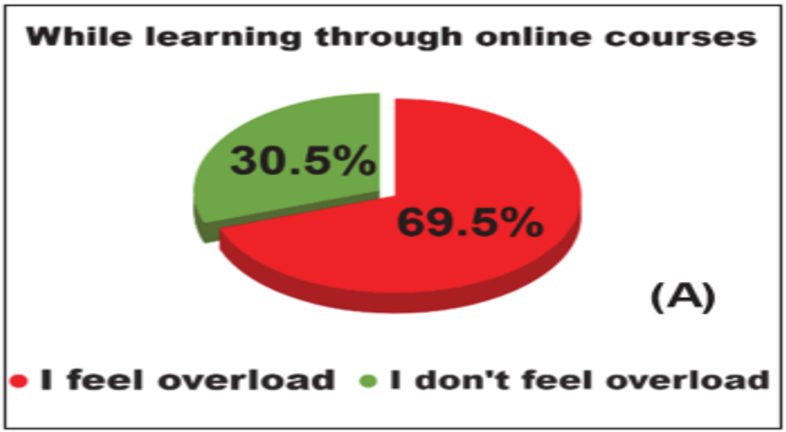
\includegraphics[scale=0.6]{pic3}
	\end{figure}

	\begin{figure}[H]
		\centering
		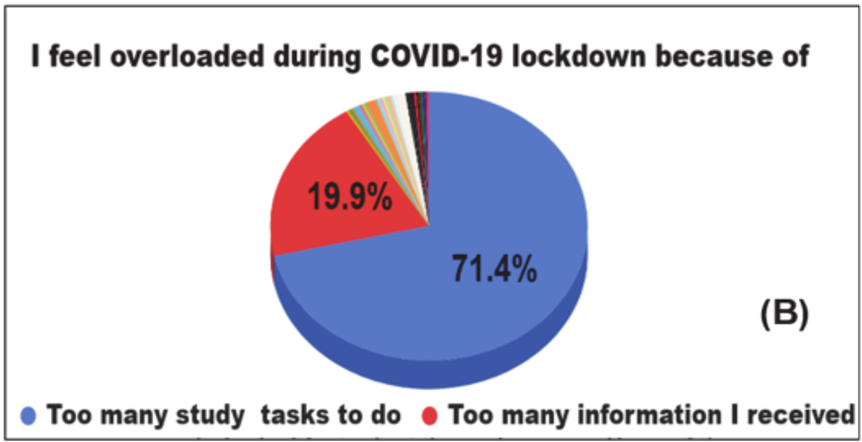
\includegraphics[scale=0.6]{pic4}
	\end{figure}

	\begin{figure}[H]
		\centering
		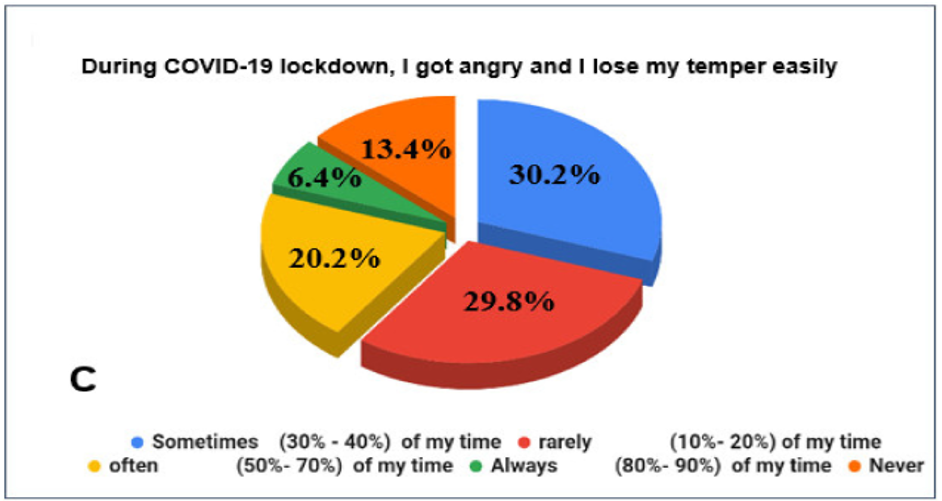
\includegraphics[scale=0.6]{pic5}
	\end{figure}

	\begin{figure}[H]
		\centering
		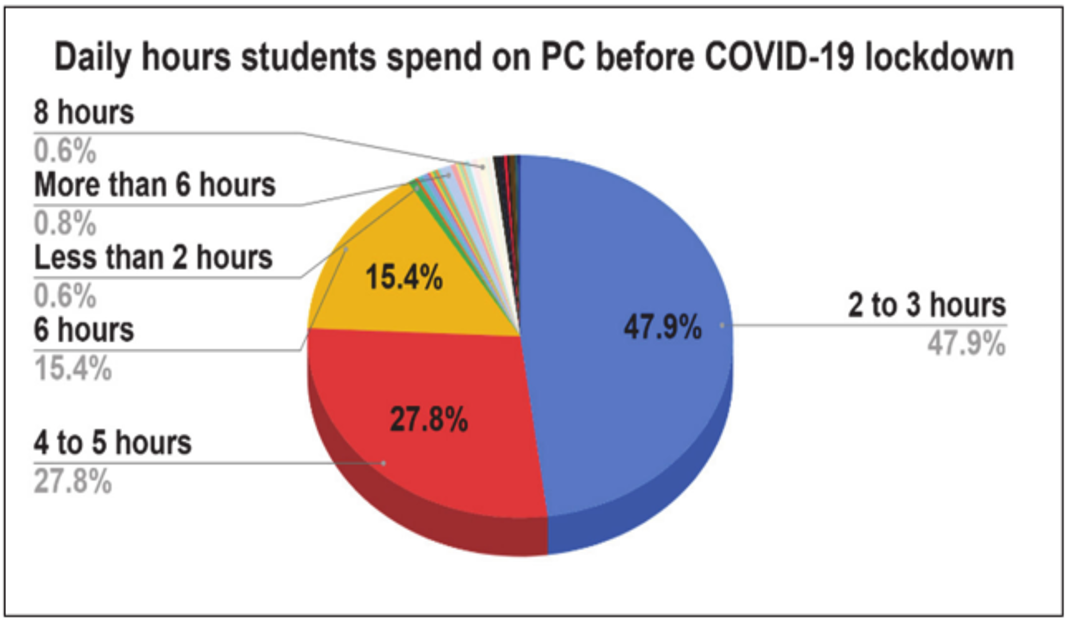
\includegraphics[scale=0.6]{pic6}
	\end{figure}

	\begin{figure}[H]
		\centering
		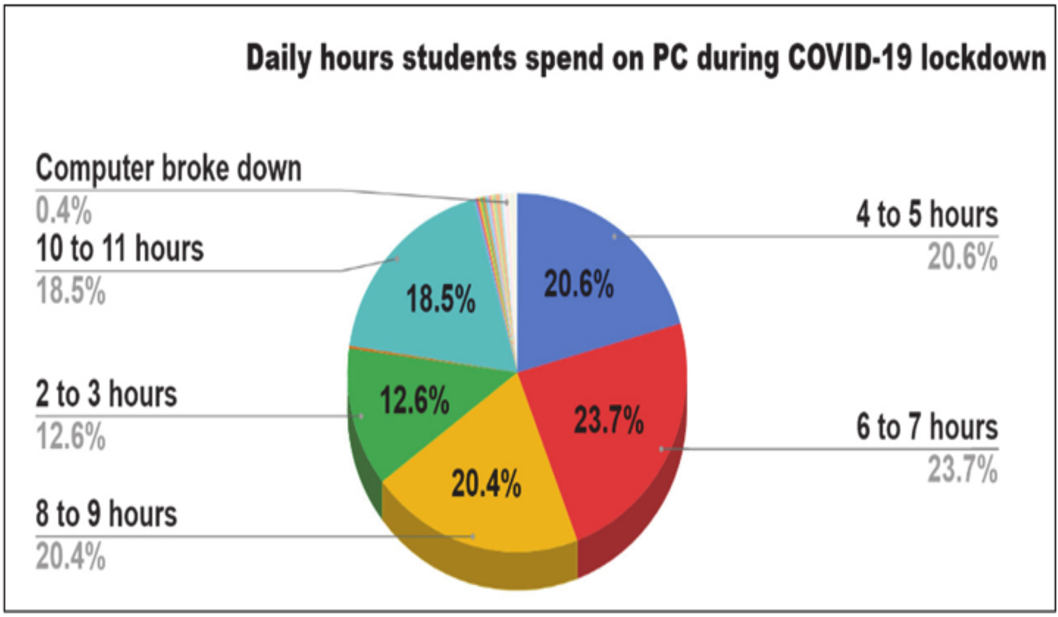
\includegraphics[scale=0.6]{pic7}
	\end{figure}

\pagebreak

	\section{Conclusion}
	
	As policymakers and educators prepare to restart schools in the midst of the COVID-19 pandemic, it is imperative that we transform our ideas of school to match the demands of this historic moment. It is clear that returning to business as usual in education is not possible and that we must think of “school” in deeply different ways. Irrespective of the approach taken to instruction or the medium through which it takes place—online, in person, or a hybrid—policymakers and educators need to ensure that all children, regardless of income, can participate in supportive and meaningful learning experiences. 
	
	This report provides an overarching framework to inform the restart of schools for the 2020–21 school year while also providing a long-term vision that can guide leaders toward new and enduring ways to address educational quality and inequity. Building upon other student-centred, equity-oriented guidance that has been developed, this framework synthesizes key ideas, evidence, state and local examples, and policy recommendations and organizes them within a broader framework focused on authentic learning and equity and grounded in research spanning early childhood through secondary schooling. It is our hope that this work will help enable state, district, and school leaders along with educators to seize this moment to strengthen learning opportunities and close opportunity and achievement gaps.
	
	\section{References}
	
	\begin{enumerate}
		\item https://www.researchgate.net/publication/350382831
		
		\item https://journals.sagepub.com/doi/full/10.1177/2347631120983481
		
		\item https://images.app.goo.gl/SRNid7PQBBhK9UA76
		
		\item https://images.app.goo.gl/tHtMCYiPYrH3HCHKA
		
		\item https://images.app.goo.gl/rByfmz3cG5hTNeEp7
		
		\item learningpolicyinstitute.org (restarting and reinventing school)
		
		\item www.unicef.org
		
		\item sustainability-13-02546-v2.pdf
		
	\end{enumerate}
\end{document}